%--------------------------------------------------------------------------------------
% Este arquivo contém a sua funtamentação teórica
%--------------------------------------------------------------------------------------
\chapter{Fundamentação teórica}

Este trabalho tem sua fundamentação no Desenvolvimento Orientado a Comportamento (BDD), com foco em sua adapatção para aplicação em desenvolvimento de sistemas de software automotivo. 
Esse processo será aplicado na definição, implementação e validação de um sistema de travamento de portas veicular.

\section{\textbf{Desenvolvimento Orientado a Comportamento - BDD}}

A metodologia de desenvolvimento orientado a comportamento foi inicialmente proposta por Dan North \cite{north2006bdd}, que compartilhou em seu blog as lições 
aprendidas ao aplicar e ensinar o processo de desenvolvimento orientado a testes (TDD). Segundo o autor, o BDD evoluiu além de práticas ágeis e é designado 
para fazê-las mais acessíveis e efetivas para times que são novos no desenvolvimento ágil.

A evolução do processo de BDD foi impulsionada por diversas descobertas práticas que surgiram em resposta às dificuldades enfrentadas na aplicação do TDD. A mudança 
da nomenclatura de ``teste'' para ``comportamento'', por exemplo, é aparentemente simples, mas gerou um impacto profundo. Essa nova terminologia ajudou a consolidar a 
ideia de que os testes devem sempre validar o comportamento esperado do sistema, o que, por sua vez, reduziu significativamente dúvidas comuns entre desenvolvedores 
iniciantes.

Outra mudança importante nesse processo foi a adoção do termo \textit{should} (deveria) em vez de \textit{shall} (deve) ou \textit{will} (vai) na formulação dos nomes 
dos testes. Desta forma, o teste se torna uma sentenção natural e provoca o questionamento se o comportamento demonstrado deveria ser realizado pelo sistema.  
Esse tipo de reflexão é especialmente valioso em equipes ágeis \cite{atlassianAgileTeams}, pois estimula o diálogo - principalmente em discussões que envolvem 
profissionais com diferentes níveis de conhecimento técnico ou de domínio do negócio.

O processo consolidado por Dan North tem foco no desenvolvimento robusto e traz diversas práticas voltadas à entregar valor ao usuário de forma mais rápida. Esse 
amadurecimento é evidente nas características apontadas por \citeonline{studyBDD} sobre o processo de BDD em sua forma atual, que consistem de:

\begin{enumerate}
	\item \textbf{Linguagem Ubíqua} - uma linguagem comum compreensível tanto por desenvolvedores quanto por especialistas do domínio ou do negócio. Deve ser utilizada 
	ao longo de todo o processo de desenvolvimento do produto, assegurando uma comunicação clara e evitando ambiguidades entre as partes envolvidas;
	\item \textbf{Processo de decomposição iterativa} - facilita a priorização do desenvolvimento de funcionalidades para o sistema ao delinear o valor gerado para o cliente final;
	\item \textbf{Descrições em texto simples com histórias de usuário e templates de cenários} - emprega templates que contém uma mistura de palavras chaves e linguagem natural na 
	criação de histórias de usuário e de cenários, garantindo sua acessibilidade e facilidade de entendimento;
	\item \textbf{Testes de aceitação automatizados com regras de mapeamento} - aplica especificações executáveis na forma de cenários compostos de passos que são traduzidos em testes, 
	os quais orientam o desenvolvimento.
\end{enumerate}

A validação das funcionalidades definidas durante o processo de BDD, consiste na criação de especificações executáveis na forma de cenários que servem de critérios de aceitação das 
histórias de usuário. Os cenários utilizam um padrão de escrita que incorpora uma junção de palavras-chave com linguagem natural e podem ter interface com o código desenvolvido por 
meio de diversas ferramentas como \textit{JBehave}, \textit{RSpec} \cite{cucumberHistory} e a que será aplicado neste trabalho - Cucumber \cite{cucumberDocs} em junção com a biblioteca 
do Python chamada Behave \cite{behaveDocs}.

% Para garantir que todas as características listadas sejam capturadas neste trabalho, o uso de histórias de usuário \cite{atlassianUserStories} e da 
% linguagem \textit{Gherkin} (Cucumber) \cite{cucumberHistory} serão aplicadas.

\section{\textbf{Definição das funcionalidades do sistema por meio de Histórias de Usuário e Mapeamento de Exemplos}}

Segundo \citeonline{atlassianUserStories}, histórias de usuário são ``uma explicação informal de uma funcionalidade de software escrita na perspectiva do usuário''. Elas 
representam uma unidade de trabalho, um objetivo de desenvolvimento a ser alcançado e garante que a equipe seja capaz de colaborar e trazer soluções inovadores 
com o usuário final em foco.

Para isso, adota-se um formato que se utiliza de linguagem natural e assegura a definição de três elementos fundamentais:

\begin{itemize}
	\item Quem é o usuário?
	\item Qual funcionalidade deve ser implementada?
	\item Qual valor essa funcionalidade traz ao usuário?
\end{itemize}

Esses três pontos são organizados em uma estrutura padronizada que utiliza conjunções específicas, resultando no seguinte modelo:
\textit{``Como [tipo de usuário], eu quero [funcionalidade], para que [valor gerado].''}
Assim como destacado por Dan North ``[...] sua força está em forçar que você identifique o valor de entregar uma história quando você a define [...]'' 
\cite{north2006bdd}. Essa ênfase em entender o valor entregue ao usuário - desde a formulação das histórias - é essencial para garantir que as funcionalidades 
desenvolvidas estejam alinhadas com as reais necessidades do usuário. 
%Durante a etapa \ref{sbs:etapa1}, serão definidas as histórias de usuário que descrevem as funcionalidades implementadas neste trabalho.

Para garantir um bom fluxo nas discussões durante a definição do escopo das histórias, o exemplo prático da aplicação de BDD demonstrado em \citeonline{Lawrence2019cucumber} 
destaca o uso do mapeamento de exemplos como uma forma eficaz para explorar e esclarecer os comportamentos esperados do sistema. Esse método contribui para que 
toda a equipe tenha uma compreensão da funcionalidade em questão e evita desvios no foco da conversa.

Dessa maneira, a definição dos comportamentos deve ser feita por meio de discussões que incluem toda a equipe e começa com citações de exemplos de uso real, priorizando 
os cenários de \textit{happy path} - aqueles em que o sistema se comporta conforme o esperado em condições normais. Estes exemplos devem ser sempre descritos a partir da 
perspectiva do usuário e podem ser trazidos de forma iterativa, sem a necessidade de que todos os casos estejam definidos antes do início do desenvolvimento.

Neste estágio do processo, existem ainda muitas incertezas acerca do sistema, o que pode dificultar a definição de comportamentos concretos que sustentem 
tecnicamente os exemplos levantados. Essa dificuldade é ainda maior quando não se tem uma descrição física do produto final ou detalhes de implementação - como no 
caso deste trabalho onde o mecanismo do travamento da porta ainda não está definido durante a etapa de mapeamento de exemplos.

Para lidar com tantos pontos desconhecidos durante discussões com a equipe, costuma-se aplicar o mapeamento de exemplos com o uso de notas adesivas coloridas, 
assim como descrito na metodologia de \citeonline{cucumberExampleMapping}. Ela se utiliza de notas coloridas em 4 cores diferentes que representam diferentes pontos:

\begin{itemize}
	\item \textbf{Amarelo}: História de usuário ou funcionalidade;
	\item \textbf{Azul}: Regra de funcionamento da história;
	\item \textbf{Verde}: Exemplo concreto que demonstra uma regra;
	\item \textbf{Vermelho}: Pergunta que foge do escopo da discussão e que deve ser investigada futuramente.
\end{itemize}

Dessa maneira, todos os pontos desconhecidos que foram previamente identificados são registrados como perguntas, evitando que a discussão se desvie para tópicos 
fora do escopo naquele momento. Essas questões são respondidas após a conclusão do mapeamento de exemplos, com base na bibliografia disponível.

Após as dúvidas serem anotadas, a discussão segue focada na experiência do usuário, mesmo que alguns aspectos técnicos ainda não estejam totalmente esclarecidos. 
Neste caso, assume-se que o veículo existe e que suas portas funcionam ``magicamente'', conforme os comportamentos definidos, permitindo que a discussão possa ser 
prosseguida com os exemplos concretos que devem ser descritos usando as notas verdes.

%\textbackslash imagem\{ Escala \}\{ Arquivo sem extensão \}\{ Descrição \}\{ Fonte \}

%\textbf{Obs.:} A fonte pode ser uma citação do tipo  \textbackslash citeonline\{\}.

% A figura \ref{img:placeholder} é um exemplo deste método.

% %--------------------------------------------------------------------------------------
% % Esse é um exemplo de figura simples
% %--------------------------------------------------------------------------------------
% \imagem{0.15}{placeholder}{Uma figura simples}{O autor}

% A figura \ref{img:figura1} é um exemplo do outro tipo de figura abordada aqui, chamada de figura composta. Esta figura é composta de outras subfiguras.
% %--------------------------------------------------------------------------------------
% % Esse é um exemplo de figura composta de outras subfiguras
% %--------------------------------------------------------------------------------------
% \begin{figure}[!htb]
% \centering
%     \caption{\label{img:figura1} Exemplo de figura composta}
%     \subcaptionbox{\label{img:subfigura1} Subfigura 1}{\includegraphics[scale=.1]{img/placeholder}}\qquad
%     \subcaptionbox{\label{img:subfigura2} Subfigura 2}{\includegraphics[scale=.1]{img/placeholder}}
%     \vspace{1.5em}
%     \legend{\textbf{Fonte:} \citeonline{SUA-REFERENCIA}}
% \label{fig:dag}
% \end{figure}

%\begin{figure}[!htb]
%\centering
%    \caption{\label{img:telas} Telas da aplicação cliente}
%    \subcaptionbox{\label{img:inicial} Abertura}{\includegraphics[scale=.12]{img/APP/inicial}}\qquad
%    \subcaptionbox{\label{img:login} \textit{Login}}{\includegraphics[scale=.12]{img/APP/login}}\qquad
%    \subcaptionbox{\label{img:cadastro} Cadastro}{\includegraphics[scale=.12]{img/APP/cadastro}}\qquad
%    \subcaptionbox{\label{img:hist-rel}Sobre}{\includegraphics[scale=.12]{img/APP/sobre}}\\
%    \vspace{1.5em}
%    \subcaptionbox{\label{img:dados_atuais}Dados atuais}{\includegraphics[scale=.15]{img/APP/atual}}\qquad
%    \subcaptionbox{\label{img:hist-time}Seleção de período}{\includegraphics[scale=.15]{img/APP/periodo}}\qquad
%    \subcaptionbox{\label{img:hist-rel}Exibir histórico}{\includegraphics[scale=.15]{img/APP/historico}}\\
%    \vspace{2.5em}
%    \legend{\textbf{Fonte:} O Autor}
%\label{fig:dag}
%\end{figure}

% \begin{figure}[ht]
% \centering
% 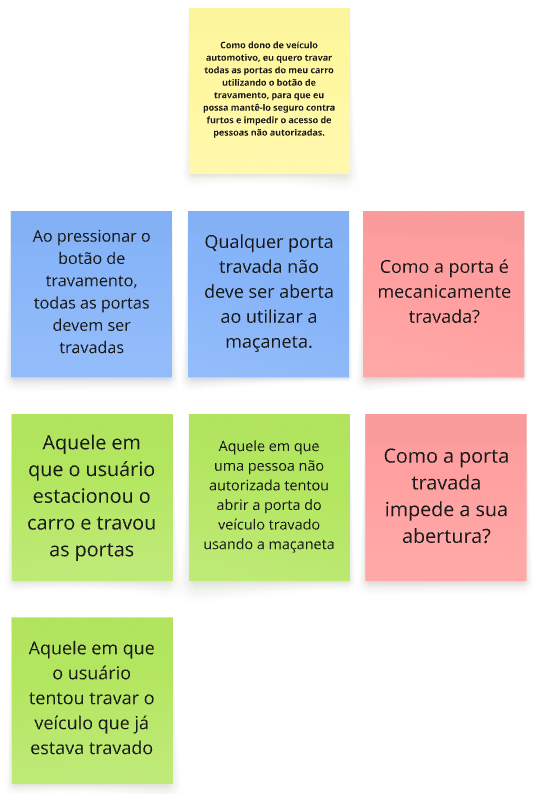
\includegraphics[height=12cm]{figuras/user_story_1.png}
% \caption{História de Usuário 1: Travamento de todas as portas}
% %\label{fig:casos-uso}
% \end{figure}

% \begin{figure}[ht]
% \centering
% 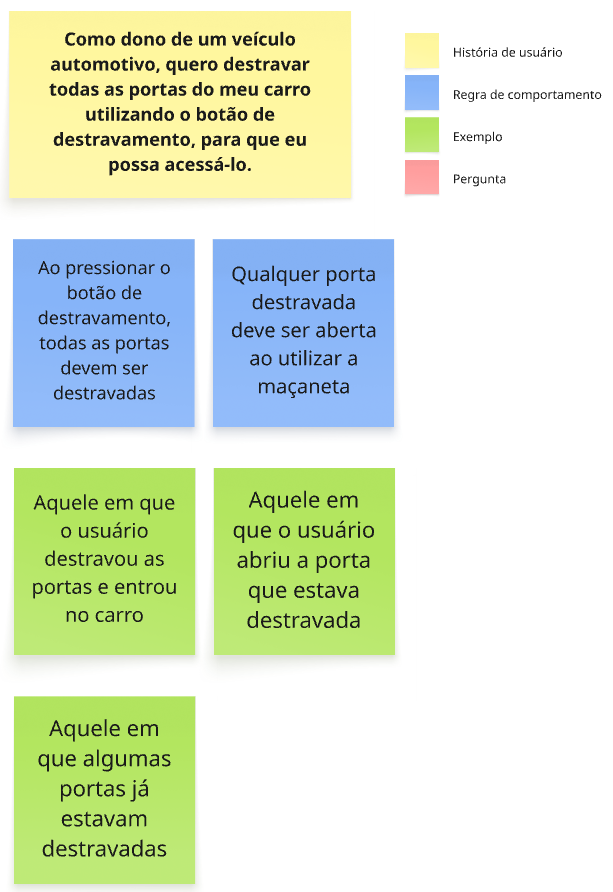
\includegraphics[height=12cm]{figuras/user_story_2.png}
% \caption{História de Usuário 2: Destravamento de todas as portas}
% %\label{fig:casos-uso}
% \end{figure}

% \begin{figure}[ht]
% \centering
% 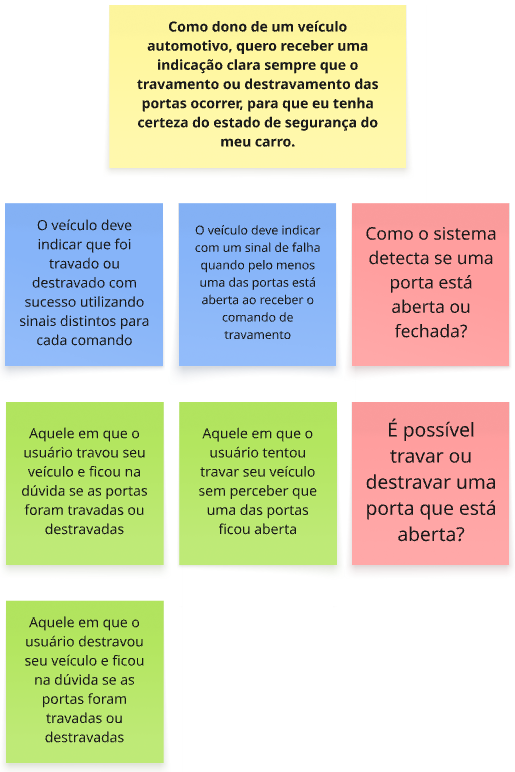
\includegraphics[height=12cm]{figuras/user_story_3.png}
% \caption{História de Usuário 3: Feedback de travamento}
% %\label{fig:casos-uso}
% \end{figure}

% \begin{figure}[ht]
% \centering
% 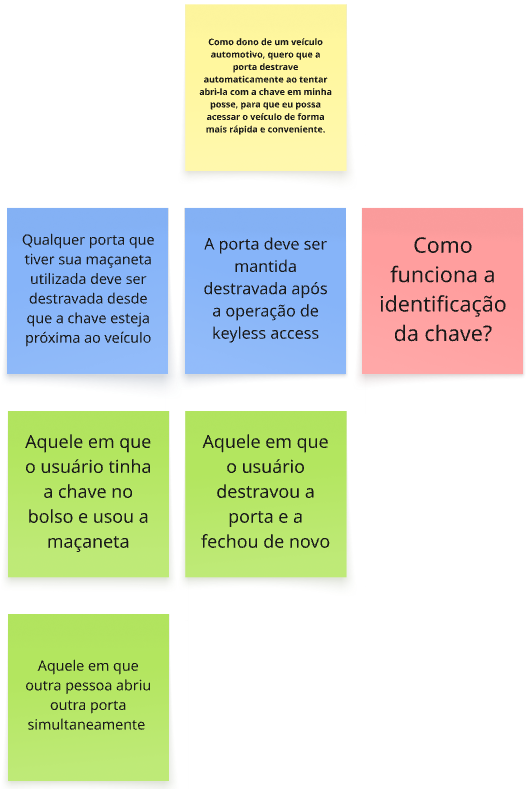
\includegraphics[height=12cm]{figuras/user_story_4.png}
% \caption{História de Usuário 4: Keyless Access}
% %\label{fig:casos-uso}
% \end{figure}

% \begin{figure}[ht]
% \centering
% 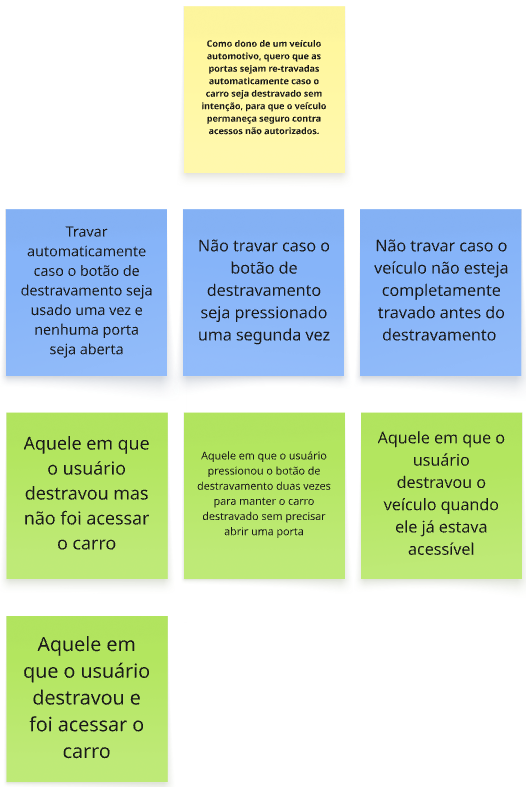
\includegraphics[height=12cm]{figuras/user_story_5.png}
% \caption{História de Usuário 5: Travamento automático}
% %\label{fig:casos-uso}
% \end{figure}

%Para referenciar uma figura deve ser usada comando \textbackslash ref\{img:<label ou nome do arquivo>\}, como exemplo, estamos referenciando a figura \ref{img:placeholder}. Isso vale tanto para figuras simples quanto para as compostas, como por exemplo as figuras \ref{img:subfigura1} e \ref{img:subfigura2}. Ao inserir uma figura, ela é automaticamente identificada e incluída no elemento pré-textual da lista de figuras.

\section{\textbf{A linguagem Gherkin}}
A linguagem \textit{Gherkin} refere-se ao padrão definido pelo \textit{Cucumber} \cite{cucumberDocs} para a escrita dos cenários do BDD. Sua estrutura baseia-se no uso das palavras-chave 
\textit{Given/When/Then} (Dado que/Quando/Então), juntamente com linguagem natural para tornar os cenários compreensíveis tanto para humanos quanto para máquinas. 

A estrutura dos cenários é organizada em arquivos com extensão \textbf{.feature}, próprios do \textit{Cucumber}. Esses arquivos contém conjuntos de cenários que descrevem os seguintes componentes do teste:

\begin{itemize}
	\item \textit{Given} - estado inicial ou pré-condições.
	\item \textit{When} - evento ou transição de estado.
	\item \textit{Then} - estado final do sistema ou ação.
\end{itemize}

% Cada componente \textit{Given/When/Then} é denominado de passo, e é responsável por descrever uma ação que deve ser executada. O conjunto de passos do cenário forma a sequência de processos que devem ser 
% realizados durante o procedimento de teste e gera um especificação que valida um comportamento do sistema.

Cada componente \textit{Given/When/Then} é denominado passo, sendo responsável por descrever uma ação a ser executada. O conjunto de passos de um cenário constitui a sequência de processos que orienta a execução 
do teste, resultando em uma especificação capaz de validar o comportamento esperado do sistema.

Para isso, o cenário descreve como o sistema deve transitar de um estado inicial - definido pela cláusula \textit{Given} - para um estado final - especificado pelo 
\textit{Then} - em resposta a uma mudança ou evento descrito pelo \textit{When}. Um exemplo disso pode ser demonstrado da seguinte forma:

\begin{verbatim}
	Scenario: Derrubar dominós
		Given eu organizei vários dominós em pé numa fila reta
		When eu derrubar o primeiro dominó
		Then todos os dominós deveriam cair em sequência 
\end{verbatim}

Este exemplo ilustra como a gramática \textit{Gherkin} pode ser utilizada para representar um cenário real na qual dominós são enfileirados e, ao se derrubar o primeiro, 
ocorre uma reação em cadeia. Ele demonstra uma clara mudança de estado que ocorre como uma resposta ao evento que é derrubar o primeiro dominó.

Um exemplo aplicado a um sistema de software para travamento de portas - como no caso abordado neste trabalho - pode ser descrito da seguinte forma:

\begin{verbatim}
	Scenario: Travando o carro
		Given o meu carro está destravado
		When eu pressiono o botão de travamento das portas
		Then o carro deveria ser travado
\end{verbatim}

Neste exemplo, o comportamento definido é o travamento das portas, que deveria acontecer uma vez em que o evento - o pressionar do botão - é executado. Dessa maneira, o
sistema realiza a transição do estado inicial - em que o carro se econtra destravado - para o cenário final - no qual as portas estão travadas.

Os dois exemplos ilustram como o uso da linguagem natural - um dos pilares do BDD - torna as especificações mais claras e acessíveis. A combinação da leitura facilitada 
com o padrão \textit{Given/When/Then} contribui tanto para contextualizar o leitor quanto para possibilitar a visualização objetiva do comportamento esperado do sistema.

% Os passos são criados nos cenários e 
% descrevem a sequência de ações ou validações que devem ocorrer na execução do teste. 

% e para implementar a lógica desta ação, a biblioteca \textit{Behave} será utilizada neste
% trabalho. Ela faz a ligação entre um passo e uma função Python, que contém os detalhes de implementação necessários para realizar o passo. 

% que são compostos por passos 
% formados ao juntar uma palavra-chave com uma sentença em linguagem natural.

A partir dos cenários Gherkin, são gerados testes automatizados, capazes de interagir com o software e verificar seu comportamento. Isso é feito por meio de definições de passos 
que contêm as instruções necessárias para manipular o sistema e gerar situações de teste.

Com a biblioteca \textit{Behave}, as definições dos passos dos cenários podem ser implementadas por meio de funções em Python. Cada função encapsula a lógica necessária para interagir 
com o sistema e executar a ação descrita no respectivo passo.

% Assim como citado por \citeonline{studyBDD} as definições de passo e integração com o software é feita de maneira iterativa, similar ao do processo de TDD, seguindo o ciclo 
% “vermelho-verde-refatorar”. Nesse contexto, cada passo do cenário assume o papel de um teste: inicialmente, o passo falha (“vermelho”); em seguida, são feitas alterações 
% mínimas para que ele seja satisfeito (“verde”); por fim, o código é aprimorado mantendo o comportamento esperado (“refatoração”).



No exemplo da cláusula \textit{When} do último cenário descrito nesta seção, a intenção do passo é representar o pressionar do botão de travamento das portas. Essa ação pode 
ser realizada por meio da alteração do sinal de entrada do sistema que indica o estado do botão, modificando seu valor de 0 para 1. Utilizando a biblioteca Behave em 
Python, isso pode ser realizado da seguinte maneira:

\begin{verbatim}
	@when('eu pressiono o botão de travamento das portas')
	def passo_pressionar_botao_de_travamento(context):
		context.botao_trava = 1
\end{verbatim}

Onde o decorador \texttt{\textbf{@when}} especifica qual passo está sendo definido, e a função \texttt{\textbf{passo\_pressionar\_botao\_de\_travamento}} contém a lógica que
deve ser executada quando esse passo for invocado. O objeto \texttt{\textbf{context}} é amplamente utilizado na biblioteca Behave por permitir o compartilhamento de 
informações entre os passos, bem como o 
acesso a interfaces do sistema sob teste. Nesse caso, assume-se que o valor do sinal referente ao botão de travamento está armazenado no objeto \texttt{context} e pode ser 
modificado por meio de uma simples atribuição.

Na prática, existem algumas complexidades adicionais a serem tratadas na implementação dessas funções, como a determinação do método para estabelecer comunicação 
com o sistema. No entanto, a função apresentada ilustra claramente o princípio do mapeamento entre os passos descritos 
em linguagem natural e as ações que operam sobre o sistema - cada passo, ao ser executado, invoca uma função responsável por manipular o sistema de forma a aplicar o 
comportamento definido na especificação.

%%%%%%%%%
% As tabelas em Latex são deveras capciosas, por isso não serão abordadas em sua completude neste documento.

% Há um site que possui uma ferramenta interessante para ser utilizada na construção tabelas em Latex.

% \centerline{\href{https://www.tablesgenerator.com/}{ O Tables Generator } <-- Isto é um \textit{link} :D}

% Contudo, busquem entendimento sobre o assunto, pois tabelas são elementos textuais importantes e enriquecem muito o texto, quando bem construídas.

% A tabela \ref{tab:crossplatform} é um exemplo de como uma tabela pode ser construída, assim como a tabela do anexo \ref{anex:anexo1}.

% \begin{table}[!htb]
% 	\centering
% 	\caption{\label{tab:crossplatform} Tipos de aplicações e abordagens preferenciais.}
% 	\begin{adjustbox}{max width=\textwidth}
% 		\begin{tabular}{@{} p{5cm} |c|c|c| @{}}
% 		\toprule
% 		\textbf{Código da Aplicação} & \textbf{Web} & \textbf{Híbrida} & \textbf{Interpretada / Compilação Cruzada} \\ \hline

% 		\textbf{Aplicações baseadas em dados providos por um servidor} &
% 			3 & 2 & 1
% 		\\ \hline

% 		\textbf{Aplicações independentes} & 1 & 2 & 3\\ \hline

% 		\textbf{Aplicações baseadas em sensores e processamento de dados no dispositivo} & 1 & 2 & 3\\ \hline

% 		\textbf{Aplicações baseadas em sensores e processamento de dados no servidor} & 1 & 3 & 2\\ \hline

% 		\textbf{Aplicações Cliente-Servidor} & 1 & 3 & 2 \\ \bottomrule
% 	\end{tabular}
% 	\end{adjustbox}
% 	\legend{\textbf{Fonte:} \citeonline{raj2012study} (Traduzido)}
% \end{table}

% Também é possível criar quadros, que são ligeiramente diferente de tabelas. Acompanhe o exemplo no Quadro \ref{qua:confusionmatrix}

% \begin{quadro}
% 	\centering
% 	\caption{\label{qua:confusionmatrix}Exemplo de matriz de confusão}
% 	\begin{tabular}{ll|c|c|}
% 		\cline{3-4}
% 		\multicolumn{1}{c}{\textbf{}} & \multicolumn{1}{c|}{\textbf{}} & \multicolumn{2}{l|}{\textbf{Classe prevista}} \\ \cline{3-4}
% 		 & \multicolumn{1}{c|}{\textbf{}} & Classe = 1 & Classe = 0 \\ \hline
% 		\multicolumn{1}{|l|}{\multirow{2}{*}{\textbf{Classe real}}} & Classe = 1 & $f_{11}$ & $f_{10}$ \\ \cline{2-4}
% 		\multicolumn{1}{|l|}{} & Classe = 0 & $f_{01}$ & $f_{00}$ \\ \hline
% 	\end{tabular}
% 	\Ididthis
% \end{quadro}


% \begin{quadro}
% 	\caption{\label{qua:cron}Cronograma}
% 	\center
% 	\begin{tabular}{|c|c|c|c|c|c|}
% 	\hline
% 	\multicolumn{1}{|l|}{Atividade} & \multicolumn{1}{l|}{Set/19} & \multicolumn{1}{l|}{Out/19} & \multicolumn{1}{l|}{Nov/19} & \multicolumn{1}{l|}{Dez/19} & \multicolumn{1}{l|}{Jan/20} \\ \hline
% 	1                               & x                           &                             &                             &                             &                             \\ \hline
% 	2                               &                             & x                           &                             &                             &                             \\ \hline
% 	3                               &                             & x                           &                             &                             &                             \\ \hline
% 	4                               &                             &                             & x                           & x                           &                             \\ \hline
% 	5                               &                             & x                           & x                           & x                           &                             \\ \hline
% 	6                               &                             &                             &                             &                             & x                           \\ \hline
	
% 	\end{tabular}
% 	\legend{\textbf{Fonte:} Elaborado pela autora (2019)}
% 	\end{quadro}

\section{\textbf{Design Orientado por Modelo}}
O desenvolvimento de software embarcado impõe uma série de desafios, conforme destacado por \citeonline{Vincentelli2001}. Entre os principais, estão os altos custos associados 
ao ciclo de desenvolvimento e as severas restrições de performance, consumo de energia e capacidade de processamento - fatores diretamente condicionados pelo 
hardware utilizado. Essas limitações tornam o processo de definição e validação do sistema particularmente complexo, já que até mesmo alterações simples nos 
requisitos podem demandar modificações significativas no código-fonte, seguidas por longas etapas de recompilação, testes e depuração.

Nesse cenário, o \textit{Model-Based Design (MBD)} surge como uma abordagem eficaz para lidar com tais dificuldades. Segundo a MathWorks \cite{mathworksMBD2024}, ele 
consiste de uma metodologia que utiliza modelos computacionais e simulações ao longo do processo de desenvolvimento de um sistema, substituindo a escrita manual 
de código. Através dessa abordagem, os sistemas podem ser projetados, simulados e validados em um ambiente integrado.

Os principais benefícios dessa metodologia são:

\begin{itemize}
	\item Ligação do design diretamente aos requisitos;
	\item Colaboração em um ambiente de desenvolvimento compartilhado;
	\item Simulação de vários cenários possíveis;
	\item Otimização de performance a nível do sistema;
	\item Geração automática de código embarcado, documentação e relatórios;
	\item Detectar erros mais cedo por testar mais cedo.
\end{itemize}

Neste trabalho o último ponto será especialmente demonstrado, devido a utilização dos testes de aceitação das histórias de usuário. Isso será feito ao integrar 
cenários \textit{Gherkin} com o modelo em \textit{Simulink} - ferramenta da MathWorks para modelagem e simulação - para executar os testes que validam o comportamento do sistema.

Outra barreira frequentemente  encontrada no desenvolvimento de software embarcado é a sua forte dependência do hardware utilizado, especialmente quando se trata 
da interação com os diversos componentes conectados ao microcontrolador. No caso do sistema de travamento de portas, por exemplo, é necessária a utilização de um 
atuador que seja capaz de acionar a trava e impedir a abertura da porta - algo que pode ser implementado com o uso de motores de passo ou servo motores.

A dificuldade surge justamente na definição das entradas e saídas do sistema, que precisam ser modeladas de forma compatível com os componentes selecionados. No 
entanto, muitas vezes o hardware ainda não está totalmente definido nesta etapa do projeto, ou pode vir a ser alterado futuramente por razões de custo, 
disponibilidade ou requisitos de desempenho. Essas mudanças forçam modificações no modelo do sistema, o que acaba reproduzindo um dos principais problemas da 
abordagem tradicional baseada em código manual: a necessidade constante de retrabalho sempre que há mudanças na base de hardware.

Para mitigar esses tipo de problema, é comum a adoção de padrões de desenvolvimento de software, como o \textit{Automotive Open System Architecture} (AUTOSAR) 
\cite{autosarClassic}, que separa o sistema em camadas, cada uma com um nível específico de abstração. Essa arquitetura em camadas permite isolar as dependências 
de hardware, facilitando a reutilização de código e a manutenção do sistema. 

No modelo AUTOSAR, a estrutura do software é decomposta nas seguintes camadas:

\begin{itemize}
	\item \textbf{Camada de Aplicação} - contém componentes de software que são responsáveis pela lógica funcional do sistema, que são completamente independentes do hardware;
	\item \textbf{Software básico} - implementa serviços que permitem o acesso direto ao hardware, lidando com os detalhes técnicos da plataforma física utilizada;
	\item \textbf{RTE (\textit{Run-Time Environment})} - faz a interface entre as duas camadas anteriores e gerencia a comunicação entre diferentes componentes de software.
\end{itemize}

Neste caso, o desenvolvimento do modelo tem foco na camada de aplicação, similar à presente no padrão AUTOSAR, definindo interfaces de entrada e saída como 
abstrações simplificadas que satisfazem o comportamento do sistema sem se prender em detalhes técnicos. Por exemplo, uma possível abstração da saída do sistema, 
considerando o problema levantado anteriormente - o estado de travamento da porta - pode ser feita ao representar cada trava por meio de um sinal binário: onde 
1 indica o estado travado e 0, o destravado. 

Essa interface corresponde à saída do modelo, a qual, na prática, é transmitida através da camada de RTE para o software básico. Nele acontece a conversão desse 
valor binário para um formato compatível com o componente físico selecionado, gerando uma interface física que é transmitida para o atuador - a trava da porta. 

\begin{figure}[H]
\centering
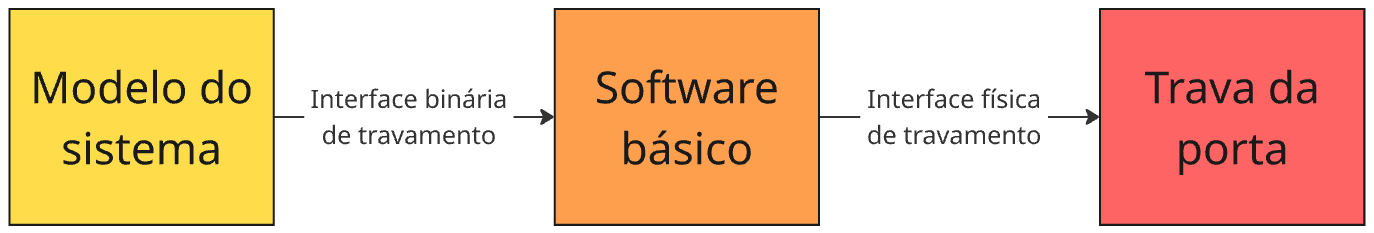
\includegraphics[height=2cm]{figuras/diagrama_interface.png}
\caption{Interfaces binárias e físicas utilizadas no travamento da porta.}
\label{fig:diagramainterface}
\end{figure}

Um benefício adicional dessa abstração é que ela permite a utilização direta das interfaces nos cenários \textit{Gherkin} e torna a validação independente dos detalhes 
técnicos do sistema, assim como é definido em testes de caixa preta \cite{sommerville2019}. Essa metodologia vai de acordo com a definição dos comportamentos no BDD, 
afinal, o valor gerado na funcionalidade de travamento de portas não depende da capacidade de movimentar um motor, mas sim da lógica que habilita o estado de travamento, 
independentemente do mecanismo utilizado para isso.

\section{\textbf{Sistemas de Travamento de Porta Veiculares}}
Segundo \citeonline{bosch2022handbook}, o sistema de travamento de portas veicular engloba todos os componentes responsáveis pelo gerenciamento do acesso ao interior 
e à saída do veículo. Sua função principal é oferecer ao motorista a possibilidade de limitar a abertura das portas, assegurando o veículo contra intrusões e acessos 
não autorizados.

Esse sistema constitui um importante recurso de conveniência e segurança, sendo capaz de realizar o travamento central \cite{reif2017locking}, que abrange não apenas 
as portas laterais, mas também o porta-malas e a tampa de acesso ao tanque de combustível. Além disso, pode incorporar diversas funcionalidades adicionais, como a 
prevenção da abertura das portas durante o uso do veículo ou o destravamento automático em situações de emergência, como em acidentes.

O mecanismo de travamento é geralmente implementado por meio de atuadores elétricos ou pneumáticos, que mantêm a porta na posição fechada e permitem, conforme a 
limitação imposta pela trava, sua abertura pelas maçanetas. Parte dos componentes estruturais do sistema é integrada à própria carroceria do veículo, como barras 
de reforço nos pilares, além dos atuadores responsáveis pelo gerenciamento das trancas. 

Para assegurar o acesso seguro ao veículo contra possíveis ataques, a autenticação da chave utiliza protocolos de criptografia \cite{glocker2016protocol}, que garantem 
a proteção tanto no registro quanto na validação das chaves. Sua implementação, conforme o padrão AUTOSAR, é realizada em um componente de software básico denominado 
\textit{Key Manager} \cite{autosarKeyManager}, o qual abstrai a metodologia empregada e disponibiliza ao software de aplicação uma interface simplificada para 
validação da chave.

A leitura da chave é normalmente feita por meio de dispositivos transceivers, responsáveis pela troca de informações com a chave utilizando tecnologias como o 
\textit{Radio Frequency Identification} (RFID) \cite{arduinoRFID}. Assim, o registro da chave indentifiacada é encaminhado ao \textit{Key Manager}, que executa 
a validação de acordo com o protocolo de criptografia definido.

Alguns fatores técnicos relevantes para a implementação física do sistema de travamento das portas e da validação das chaves serão detalhados na Seção \ref{ch:IM}, 
apresentados sob a forma de perguntas levantadas durante o mapeamento de exemplos da Etapa \ref{sbs:etapa2}. Isso se deve à natureza do processo de BDD, que prioriza 
a definição das funcionalidades a partir da perspectiva do usuário, em vez de se concentrar na tecnologia ou na metodologia empregada. Assim, a elaboração das 
histórias de usuário independe da definição prévia do mecanismo específico de travamento adotado ou do protocolo de autenticação de chaves a ser implementado.
